\documentclass[tikz]{standalone}
\usepackage{tikz,amsmath}
\begin{document}
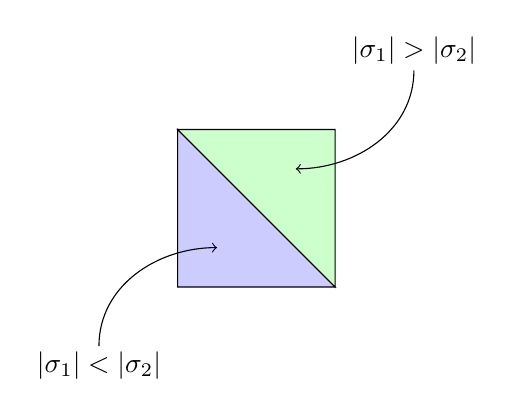
\begin{tikzpicture}[sloped]
    \draw [fill=blue!20] (0,0) -- (0,2) -- (2,0) -- cycle;
    \draw [fill=green!20] (2,2) -- (0,2) -- (2,0) -- cycle;
    \node at (3,3)  {\(|\sigma_1|>|\sigma_2|\)};
    \node at (-1,-1)  {\(|\sigma_1|<|\sigma_2|\)};
    \draw (-1, -.75) edge[out=90, in=180, ->] (.5,.5);
    \draw (3, 2.75) edge[out=-90, in=0, ->] (1.5,1.5);
\end{tikzpicture}
\end{document}
